\end{multicols}

\begin{center}
    \begin{minipage}[b]{.40\textwidth}
        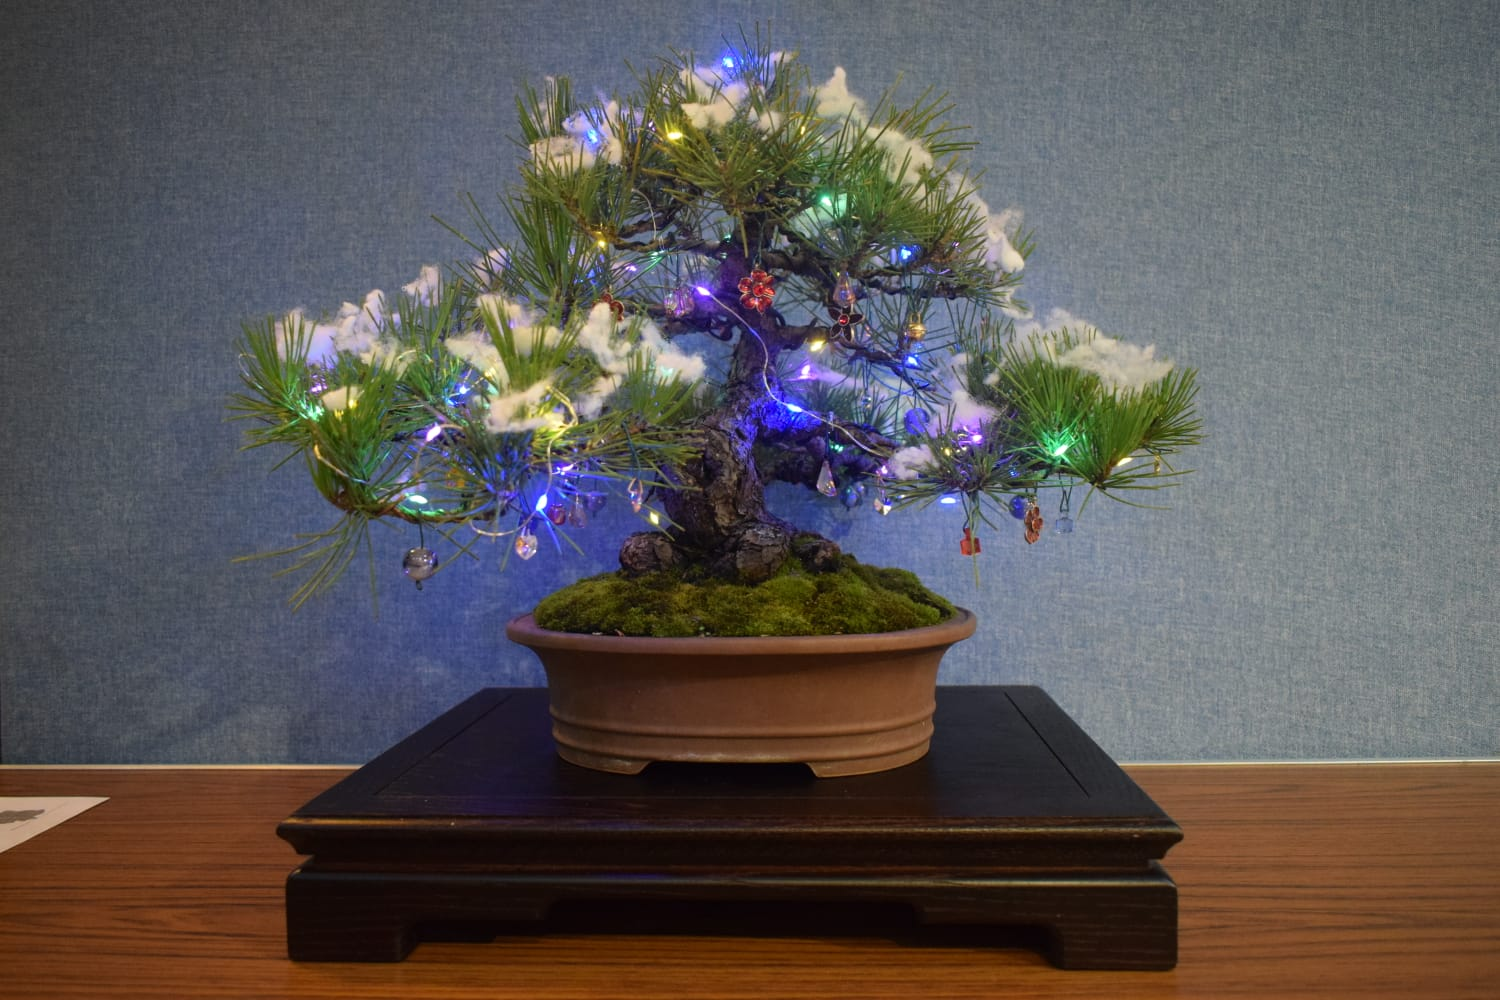
\includegraphics[angle=0,origin=c,width=1.0\textwidth]{2024_12/res/tony_pinus_nigra.jpeg}
        \centerline{\emph{Tony U's Pinus Nigra.}}
    \end{minipage}\quad
    \begin{minipage}[b]{.40\textwidth}
        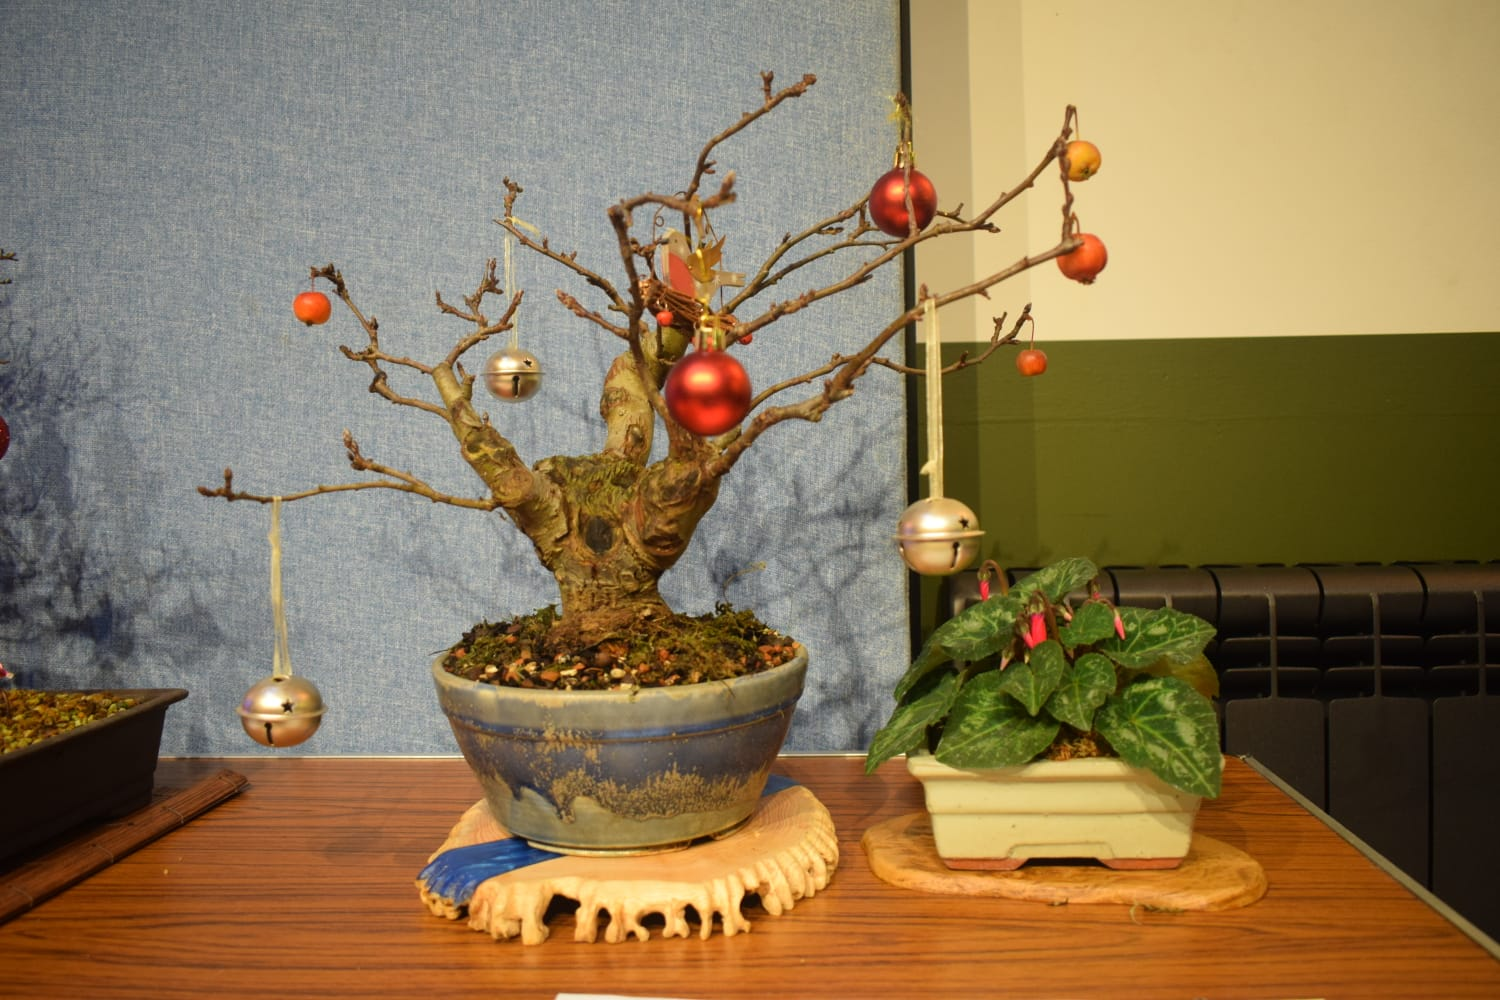
\includegraphics[angle=0,origin=c,width=1.0\textwidth]{2024_12/res/rory_crab_apple.jpeg}
        \centerline{\emph{Rory's Crab Apple.}}
    \end{minipage}

    \begin{minipage}[b]{.40\textwidth}
        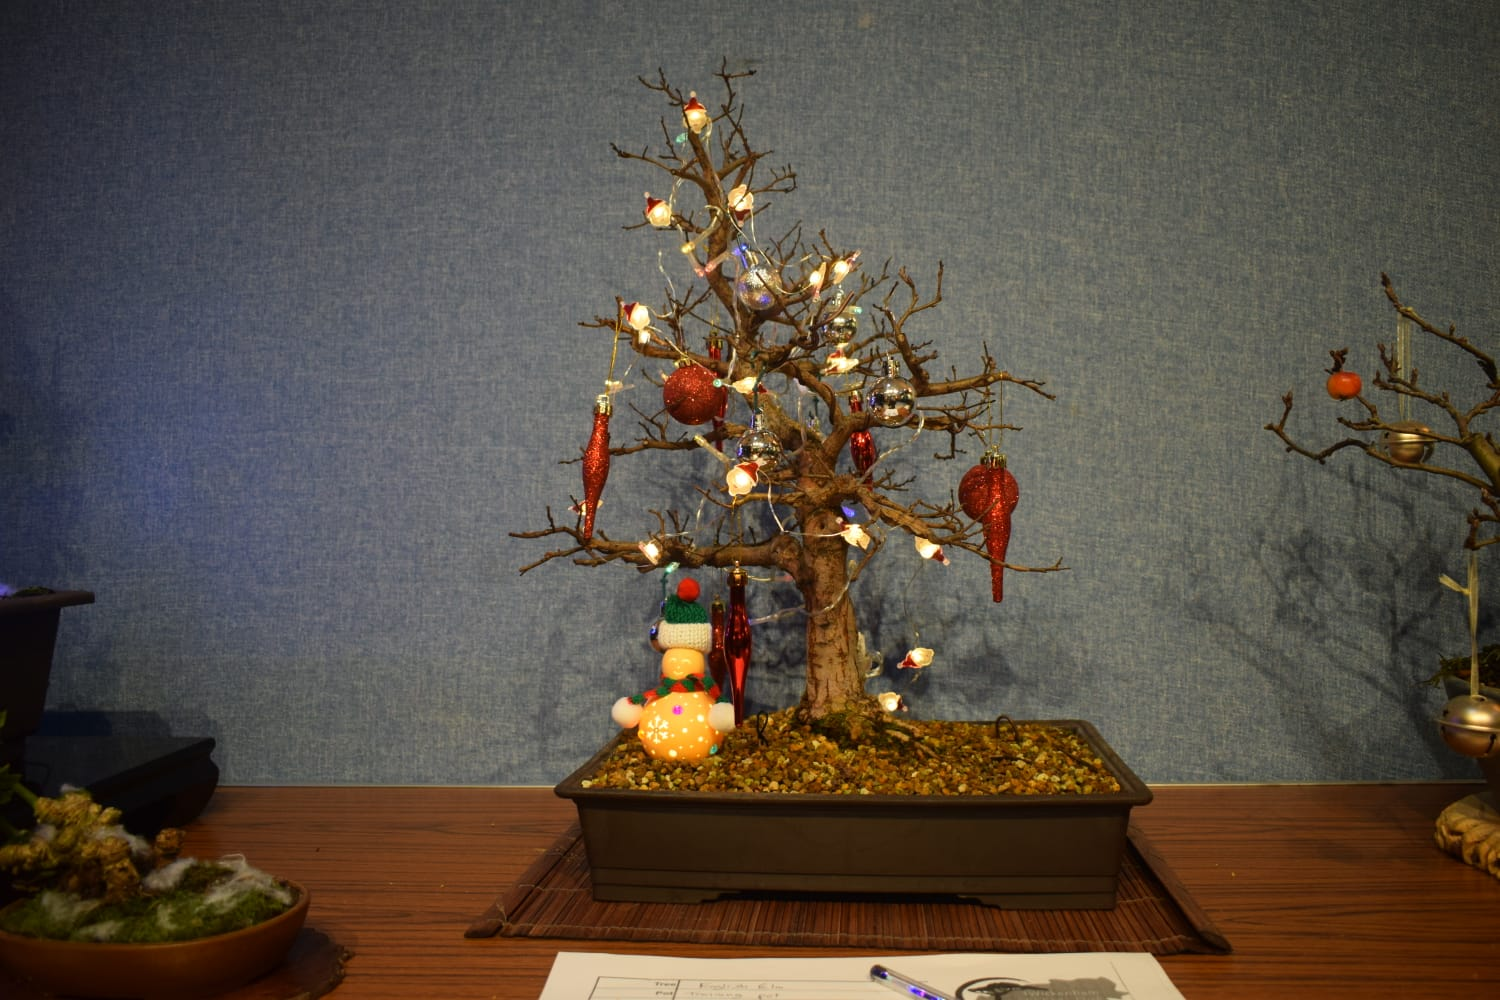
\includegraphics[angle=0,origin=c,width=1.0\textwidth]{2024_12/res/jodi_english_elm.jpeg}
        \centerline{\emph{Jodi's English Elm.}}
    \end{minipage}\quad
    \begin{minipage}[b]{.40\textwidth}
        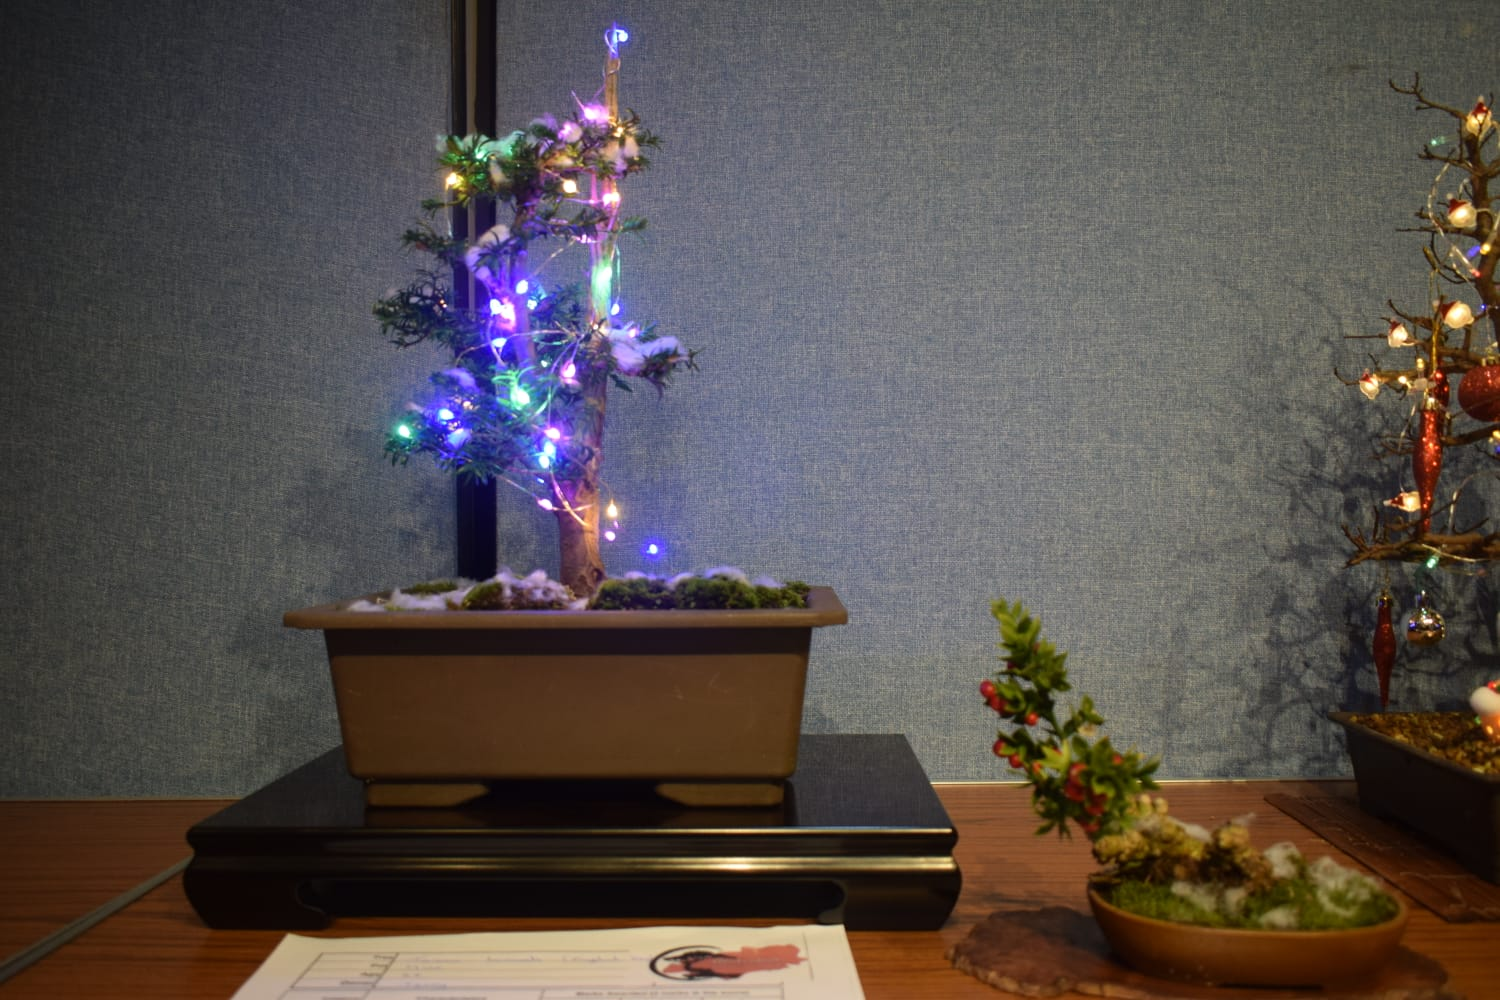
\includegraphics[angle=0,origin=c,width=1.0\textwidth]{2024_12/res/terry_english_elm.jpeg}
        \centerline{\emph{Terry's English Elm.}}
    \end{minipage}

    \begin{minipage}[b]{.25\textwidth}
        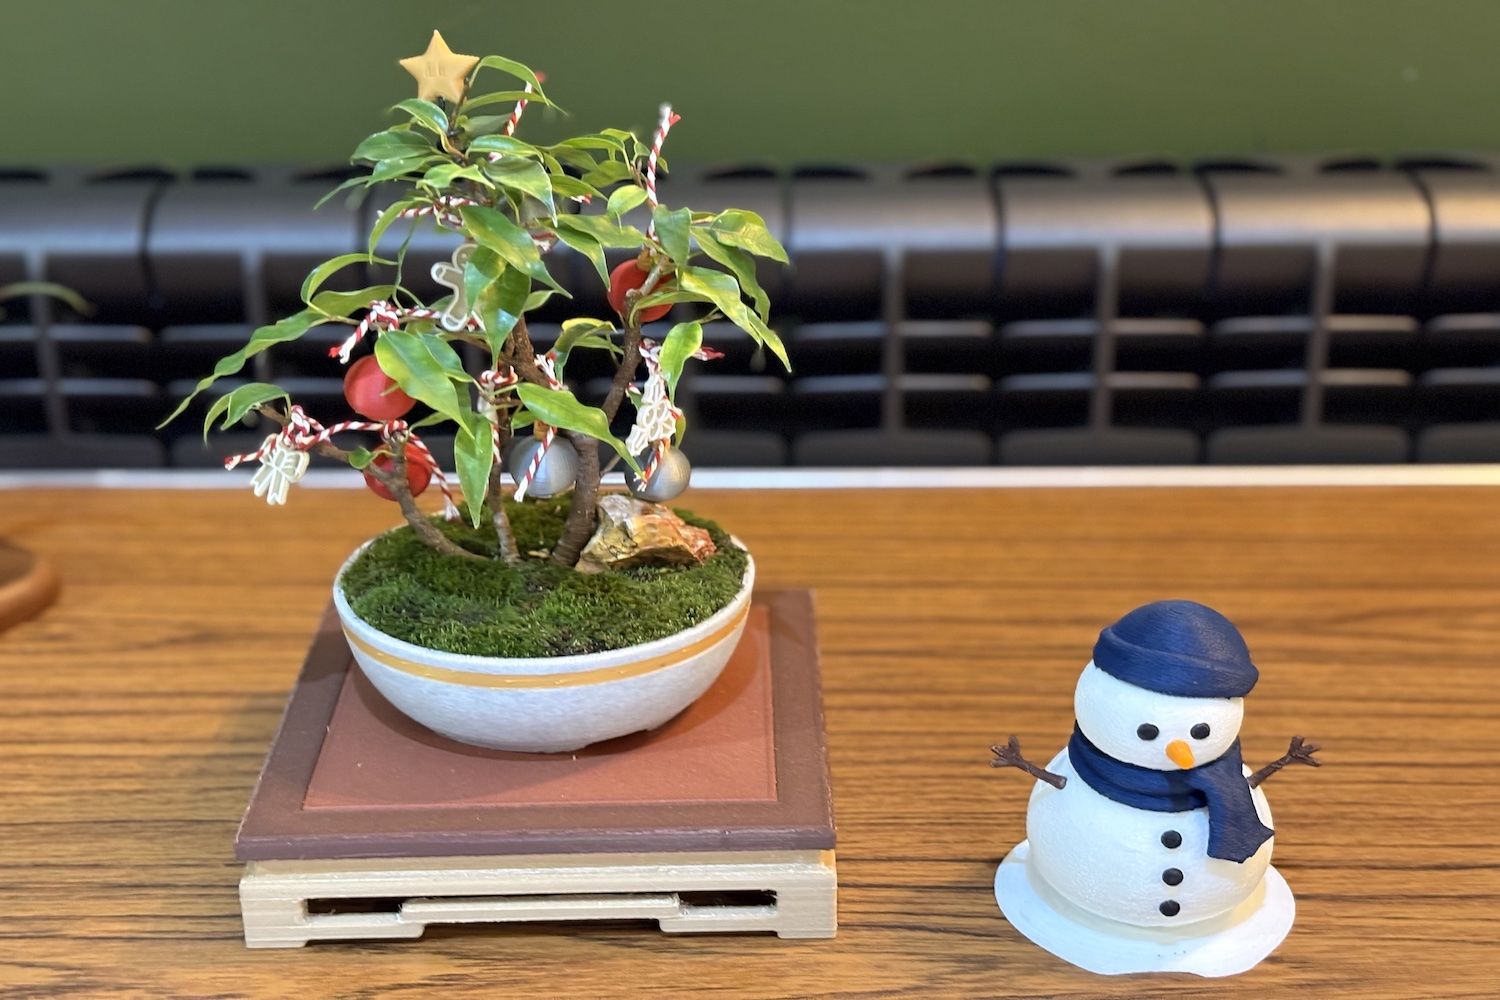
\includegraphics[angle=0,origin=c,width=1.0\textwidth]{2024_12/res/stefano_ficus_benjamina.jpg}
        \centerline{\emph{Stefano's Ficus Benjamina.}}
    \end{minipage}\quad
    \begin{minipage}[b]{.25\textwidth}
        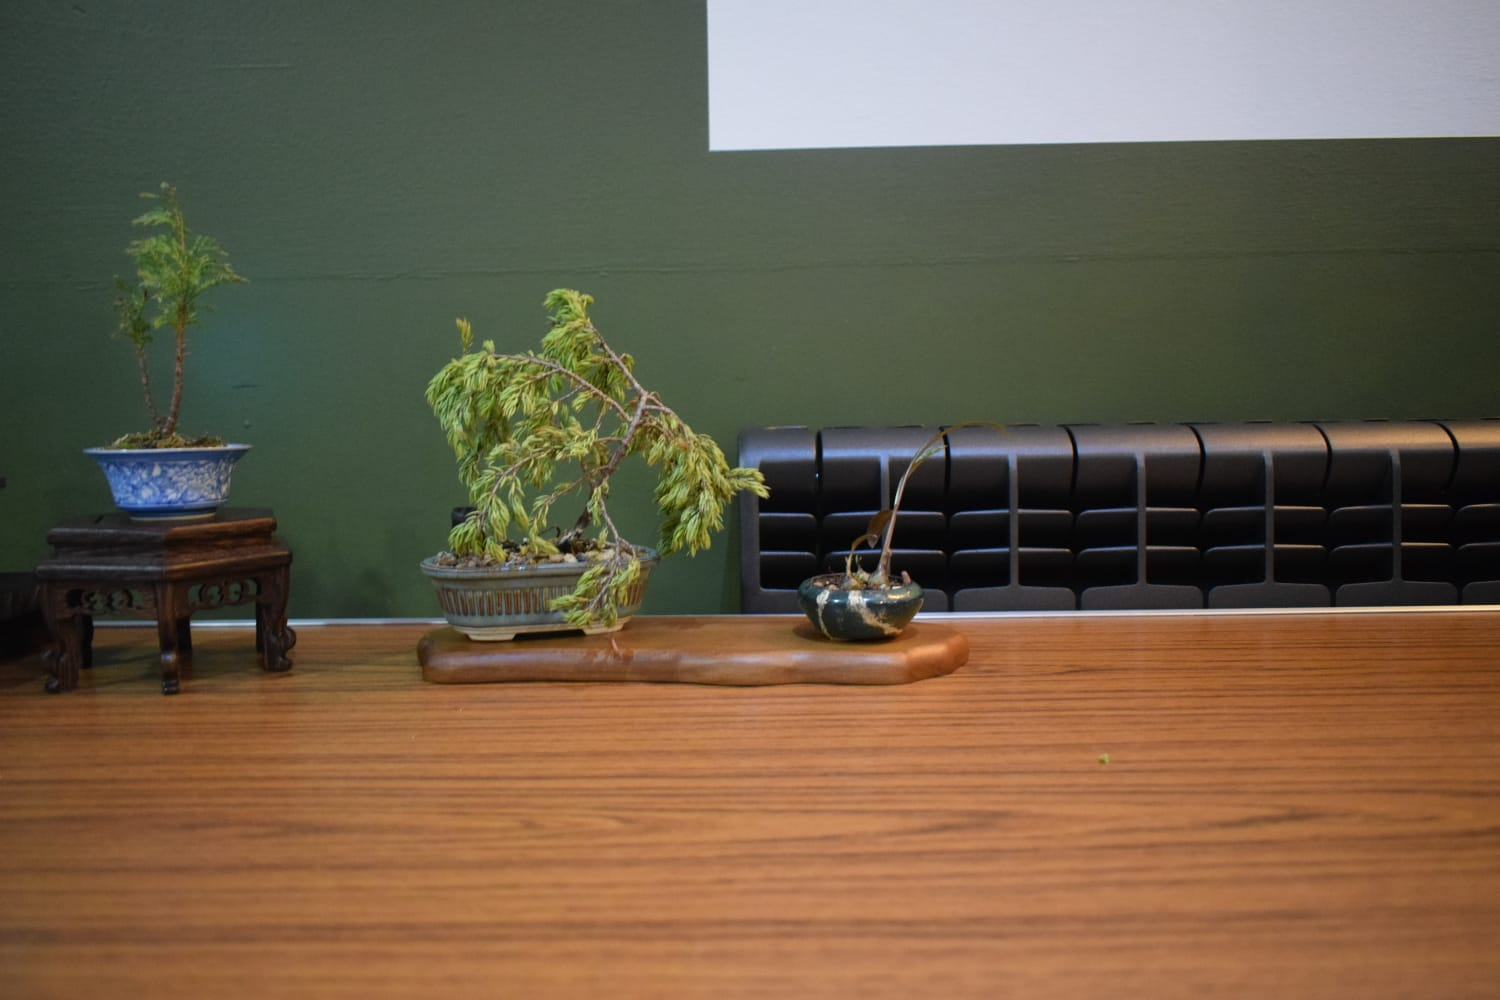
\includegraphics[angle=0,origin=c,width=1.0\textwidth]{2024_12/res/edward_pansal_pine}
        \centerline{\emph{Edwards's English Elm.}}
    \end{minipage}\quad
    \begin{minipage}[b]{.25\textwidth}
        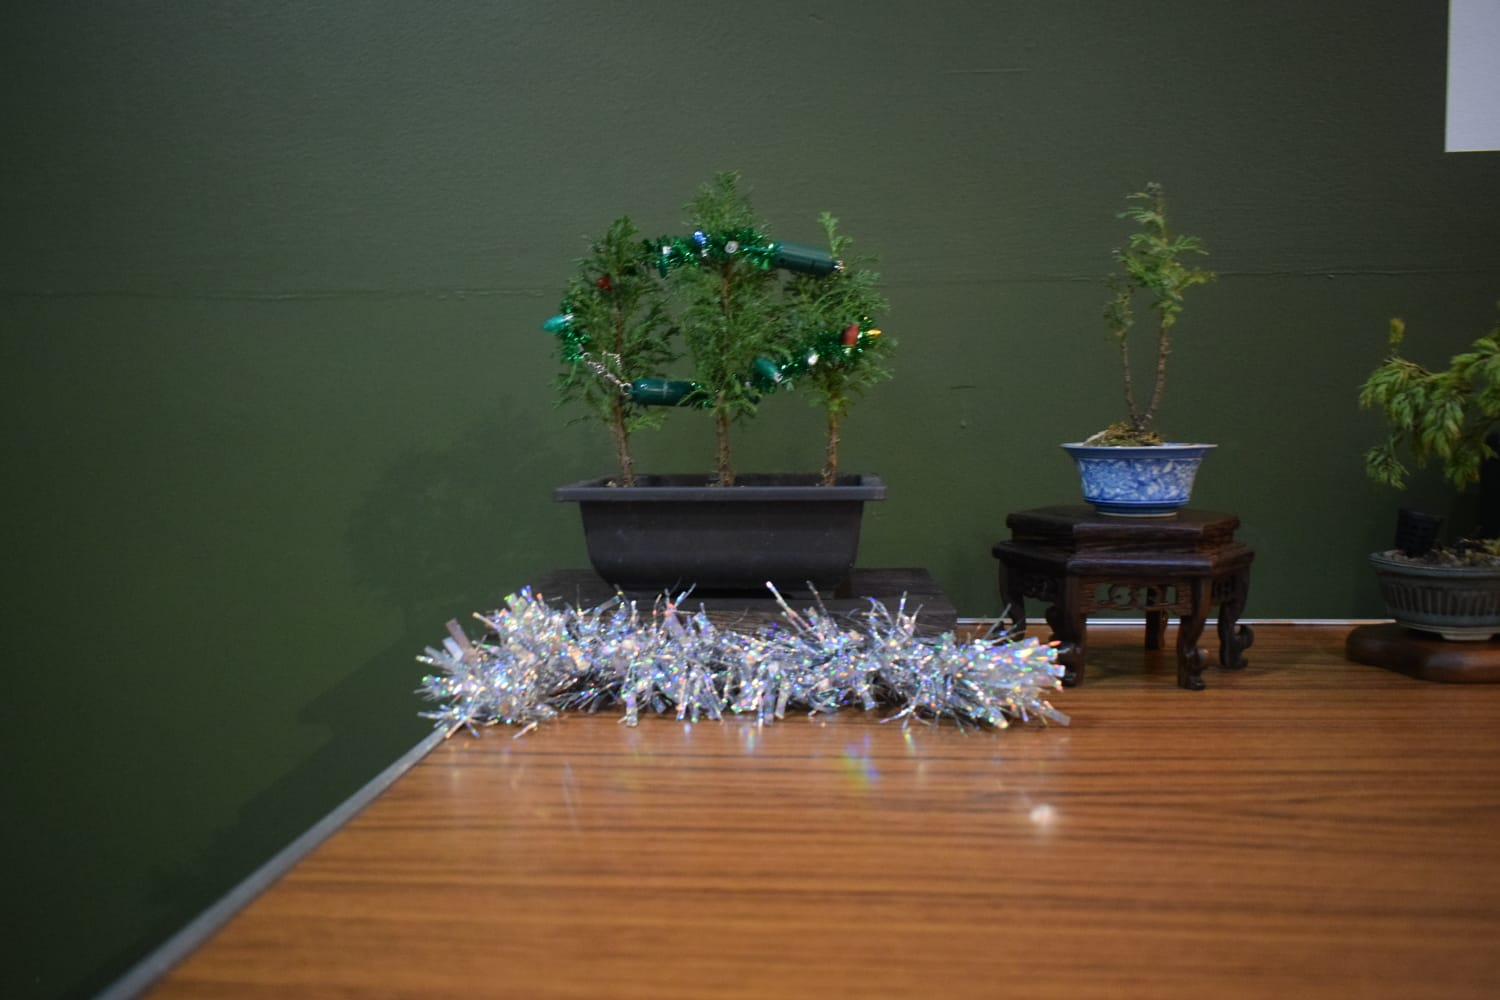
\includegraphics[angle=0,origin=c,width=1.0\textwidth]{2024_12/res/laura_juniper}
        \centerline{\emph{Laura's Juniper.}}
    \end{minipage}
\end{center}

\begin{multicols}{2}

\headline{{\textbf{\Large\sffamily The Top Chop:}}\\
          {\textbf{\large\sffamily The Tree of the Month Contest}}}
\label{2024-12-contest}
\noindent
The December Tree of the Month show brought festive cheer to the club as members showcased their finest bonsai on the theme of \textbf{Christmas Trees}.
The competition featured two categories: \textbf{Tree of the Month} for experienced members and \textbf{Novice Tree of the Month} for members with less than two years of experience.
Club members can vote on other member's trees by casting 1 to 3 marks on 4 different aspects (trunk and branches, foliage, pot/container, and presentation), for up to 12 marks per entry.

\topic{Tree of the Month}
\noindent
This month we had four submissions for Tree of the Month:

\begin{enumerate}
    \item \textbf{Tony U} dazzled with his \emph{Pinus Nigra}, earning an impressive 144 points to secure first place.

    \item \textbf{Rory}'s \emph{Crab Apple} followed with 115 points,

    \item \textbf{Jodi}'s \emph{English Elm} scored 100 points, and

    \item \textbf{Terry}'s \emph{English Elm} earned 81 points.
\end{enumerate}

% \begin{window}[0,r,
\includegraphics[width=0.45\columnwidth]{2024_12/tony_pinus_nigra}
\includegraphics[width=0.45\columnwidth]{2024_12/rory_crab_apple},\centerline{\emph{Tony U's pinus nigra (l) and Rory's crab apple (r).}}]
% \end{window}

% \begin{figure*}[h]
%   \centering
%   \subfigure[random caption 1]{
\includegraphics[scale=0.45\pagewidth]{2024_12/tony_pinus_nigra.jpg}}\quad
%   \subfigure[random caption 2]{
\includegraphics[scale=0.45\pagewidth]{2024_12/rory_crab_apple}}
% \end{figure*}

\textbf{Winner:} Tony U with his magnificent \emph{Pinus Nigra}.

\topic{Novice Tree of the Month}
\noindent
Three trees were presented as Novice Tree of the Month:

\begin{enumerate}
    \item \textbf{Stefano} entered the competition with his creative \emph{Ficus Benjamina}, scoring 77 points,

    \item \textbf{Edward}'s \emph{Pansal Pine} received 76 points, narrowly missing the win, and

    \item \textbf{Laura}'s \emph{Juniper} scored 60.
\end{enumerate}

\textbf{Winner:} Stefano with his charming \emph{Ficus Benjamina}.

Congratulations to all participants for their outstanding entries!
Be sure to prepare for next month's Tree of the Month show, where the theme will be \textbf{Indoor, Tropical, or Native Trees}.
See you then!
\closearticle
\clearpage
